\newpage
\section{文件系统}
\par 这一节的代码较多,故统一放在附录。
\subsection{实验内容}
\par 实现具有设备创建、分区格式化、注册文件系统、文件夹操作、文件操作功能的完整文件系统。

\subsection{实验环境}
\par 本实验在 Linux 6.18.0-ARCH (aarch64) 内核环境下进行。由于 Linux 内核 API 持续演进,6.x 系列内核相较于早期版本存在若干重要变化,本文档将特别标注这些差异。

\subsection{实验步骤}

\subsubsection{创建虚拟块设备}

\begin{lstlisting}[language=bash]
# 创建一个 2MB 的空文件
dd if=/dev/zero of=image bs=1k count=2000
# 关联 loop 设备
sudo losetup /dev/loop0 image
\end{lstlisting}

\par \texttt{dd}是Linux提供的数据复制工具,按块操作。在这里,我们指定它的输入源是\texttt{/dev/zero},这是一个无限产生 \texttt{0x00} 字节的虚拟设备。我们通过\texttt{of=image},将这虚拟设备产生的全零字节输出到当前目录下名为 \texttt{image} 的文件,指定每个块大小为1k,复制两千个块。这里的1k是1024个字节。

\par \texttt{losetup}是循环设备(loop device)管理工具。循环设备是一种伪设备,它允许我们将普通文件当作块设备来使用。通过\texttt{sudo losetup /dev/loop0 image},我们将刚才创建的\texttt{image}文件关联到\texttt{/dev/loop0}这个循环设备上。此后,对\texttt{/dev/loop0}的任何读写操作,内核都会将其转发到\texttt{image}文件上。这样,我们就可以像操作真实磁盘一样对这个文件进行分区、格式化和挂载操作,而无需使用真正的物理存储设备。

\par 在继续之前,有必要理解``块''这一概念。磁盘等存储设备在硬件层面并不支持逐字节访问,而是以固定大小的``块''(block)为单位进行读写。这是由硬件特性决定的:磁盘的磁头一次扫过会读取一整段数据,闪存芯片一次擦写操作也作用于整个物理块。因此,操作系统将存储设备抽象为``块设备''(block device),所有I/O操作都以块为最小单位。在本实验中,我们创建的2MB镜像文件通过循环设备被内核视为一个块设备,后续我们将在这个虚拟块设备上实现自己的文件系统。

\subsubsection{文件系统布局}

\par 在深入代码之前,我们需要理解文件系统在磁盘上的布局。一个文件系统需要存储元数据(描述文件系统本身和文件属性的数据)以及实际的文件内容。我们的简易文件系统采用如下布局:

\begin{figure}[htbp]
\centering
\begin{tikzpicture}[
    block/.style={draw, minimum width=2.5cm, minimum height=1.2cm, align=center, font=\small},
    arrow/.style={->, >=stealth, thick}
]
    % --- 绘制各个块 (基于我们的 C 代码逻辑) ---
    
    % Block 0: 代码中直接 write(fd, &sb, ...) 到开头
    \node[block, fill=blue!20] (sb) at (0, 0) {超级块\\Block 0\\(Magic: 0x114514)};
    
    % Block 1: 代码中 lseek 到 512 写入 Inode
    \node[block, fill=orange!20] (itable) at (3, 0) {Inode 表\\Block 1\\(包含 Root Inode)};
    
    % Block 2: 代码中 lseek 到 1024 写入 "." 和 ".."
    \node[block, fill=yellow!20] (rootdata) at (6, 0) {根目录数据\\Block 2\\(存 . 和 ..)};
    
    % Block 3+: 未使用区域
    \node[block, fill=gray!10, dashed] (free) at (9, 0) {空闲数据区\\Block 3+};
    
    % --- 标注连接关系 ---
    % \draw[arrow] (sb.east) -- (itable.west);
    \draw[arrow] (itable.east) -- (rootdata.west);
    \draw[arrow] (rootdata.east) -- (free.west);

    \node[below=0.2cm, red] at (sb.south) {\texttt{Offset 0}};
    \node[below=0.2cm, red] at (itable.south) {\texttt{Offset 512}};
    \node[below=0.2cm, red] at (rootdata.south) {\texttt{Offset 1024}};
    
\end{tikzpicture}
\caption{简易文件系统磁盘布局}
\label{fig:real-fs-layout}
\end{figure}

\par 超级块位于 Block 0,存储文件系统的全局元数据,包括魔数、块大小、根目录位置等关键信息,是内核识别和挂载文件系统的依据。inode 表位于 Block 1,集中存放所有文件和目录的元数据,每个 inode 描述一个文件的属性及其数据块位置。根目录的数据存储在 Block 2,包含初始的 \texttt{.} 和 \texttt{..} 目录项。Block 3-9 作为保留区,Block 10 及之后的空间构成数据区,用于存储新创建的文件和目录内容。

\subsubsection{核心数据结构}

\par 我们在头文件 \texttt{naive\_fs.h} 中定义了文件系统的三个核心数据结构。这些结构体将同时用于磁盘存储和内核模块,因此使用\texttt{\_\_le32}类型确保小端字节序,保证跨平台兼容性。

\par 超级块结构描述整个文件系统的全局信息:

\begin{lstlisting}[language=C]
#define NAIVE_MAGIC 0x114514 
#define NAIVE_BLOCK_SIZE 512
#define NAIVE_FILENAME_MAX 28

struct naive_super_block {
    __le32 magic;        // 魔数,用于识别文件系统类型
    __le32 block_count;  // 文件系统总块数
    __le32 inode_count;  // inode总数
    __le32 root_inode;   // 根目录的inode号
};
\end{lstlisting}
\par 魔数\texttt{0x114514}是文件系统的唯一标识符。当内核尝试挂载一个分区时,会读取超级块并校验魔数,以此判断分区所使用的文件系统类型。若魔数不匹配,挂载将失败。

\newpage
\par inode结构描述单个文件或目录的元数据:

\begin{lstlisting}[language=C]
struct naive_inode {
    __le32 mode;           // 文件类型与权限
    __le32 uid;            // 所有者用户ID
    __le32 gid;            // 所有者组ID
    __le32 size;           // 文件大小(字节)
    __le32 ctime;          // 创建时间
    __le32 blocks;         // 占用的块数
    __le32 data_block[10]; // 直接索引数组
};
\end{lstlisting}

\par inode是Unix文件系统的核心抽象。每个文件或目录都对应唯一的inode,存储其属性信息以及指向数据块的索引。\texttt{data\_block}数组采用直接索引方式,每个元素指向一个512字节的数据块,因此单个文件最大支持$10 \times 512 = 5120$字节。若需支持更大的文件,则需实现间接索引或多级索引机制。值得注意的是,文件名并不存储在inode中,而是存储在目录项里,这种设计使得硬链接成为可能——多个文件名可以指向同一个inode。

\par 目录项结构用于建立文件名与inode之间的映射:

\begin{lstlisting}[language=C]
struct naive_dir_entry {
    char name[NAIVE_FILENAME_MAX]; // 文件名(28字节)
    __le32 inode_no;               // 对应的inode号(4字节)
};
\end{lstlisting}

\par 目录在文件系统中本质上是一种特殊的文件,其数据块中存储的是目录项数组而非普通数据。每个目录项将一个文件名映射到对应的inode号。我们采用定长目录项设计,每项恰好32字节,这简化了目录的遍历和管理:在一个512字节的块中可以容纳$512 \div 32 = 16$个目录项。文件名长度限制为28字节,加上4字节的inode号,构成完整的32字节目录项。
\newpage
\subsubsection{格式化工具}

\par 格式化工具 \texttt{mkfs.naive} 负责在块设备上初始化文件系统的数据结构。以下是其核心实现:

\begin{lstlisting}[language=C]
int main(int argc, char *argv[]) {
    int fd = open(argv[1], O_RDWR);
    
    // 步骤 1: 写入超级块 (Block 0)
    struct naive_super_block sb = {
        .magic = NAIVE_MAGIC,
        .block_count = 2000,
        .inode_count = 100,
        .root_inode = 1,
    };
    lseek(fd, 0, SEEK_SET);
    write(fd, &sb, sizeof(sb));

    // 步骤 2: 写入根目录 Inode (Block 1)
    struct naive_inode root_inode = {
        .mode = S_IFDIR | 0755,
        .size = sizeof(struct naive_dir_entry) * 2,
        .blocks = 1,
        .data_block = { 2 }  // 指向 Block 2
    };
    lseek(fd, NAIVE_BLOCK_SIZE + sizeof(struct naive_inode), SEEK_SET);
    write(fd, &root_inode, sizeof(root_inode));

    // 步骤 3: 写入根目录数据 (Block 2)
    struct naive_dir_entry entries[2];
    strncpy(entries[0].name, ".", NAIVE_FILENAME_MAX);
    entries[0].inode_no = 1;
    strncpy(entries[1].name, "..", NAIVE_FILENAME_MAX);
    entries[1].inode_no = 1;
    
    lseek(fd, NAIVE_BLOCK_SIZE * 2, SEEK_SET);
    write(fd, entries, sizeof(entries));
    
    close(fd);
    return 0;
}
\end{lstlisting}

\par 格式化过程分三步完成。首先在 Block 0 写入超级块,设置魔数和基本参数。然后在 Block 1 的 inode 表中写入根目录的 inode(跳过保留的 inode 0,根目录使用 inode 1),其 \texttt{mode} 字段设为 \texttt{S\_IFDIR | 0755} 表示这是一个权限为 \texttt{rwxr-xr-x} 的目录,\texttt{data\_block[0]} 指向 Block 2。最后在 Block 2 写入根目录的初始内容,包含 \texttt{.}(指向自身)和 \texttt{..}(指向父目录,对于根目录来说也是自身)两个目录项。
\begin{figure}
  \begin{center}
    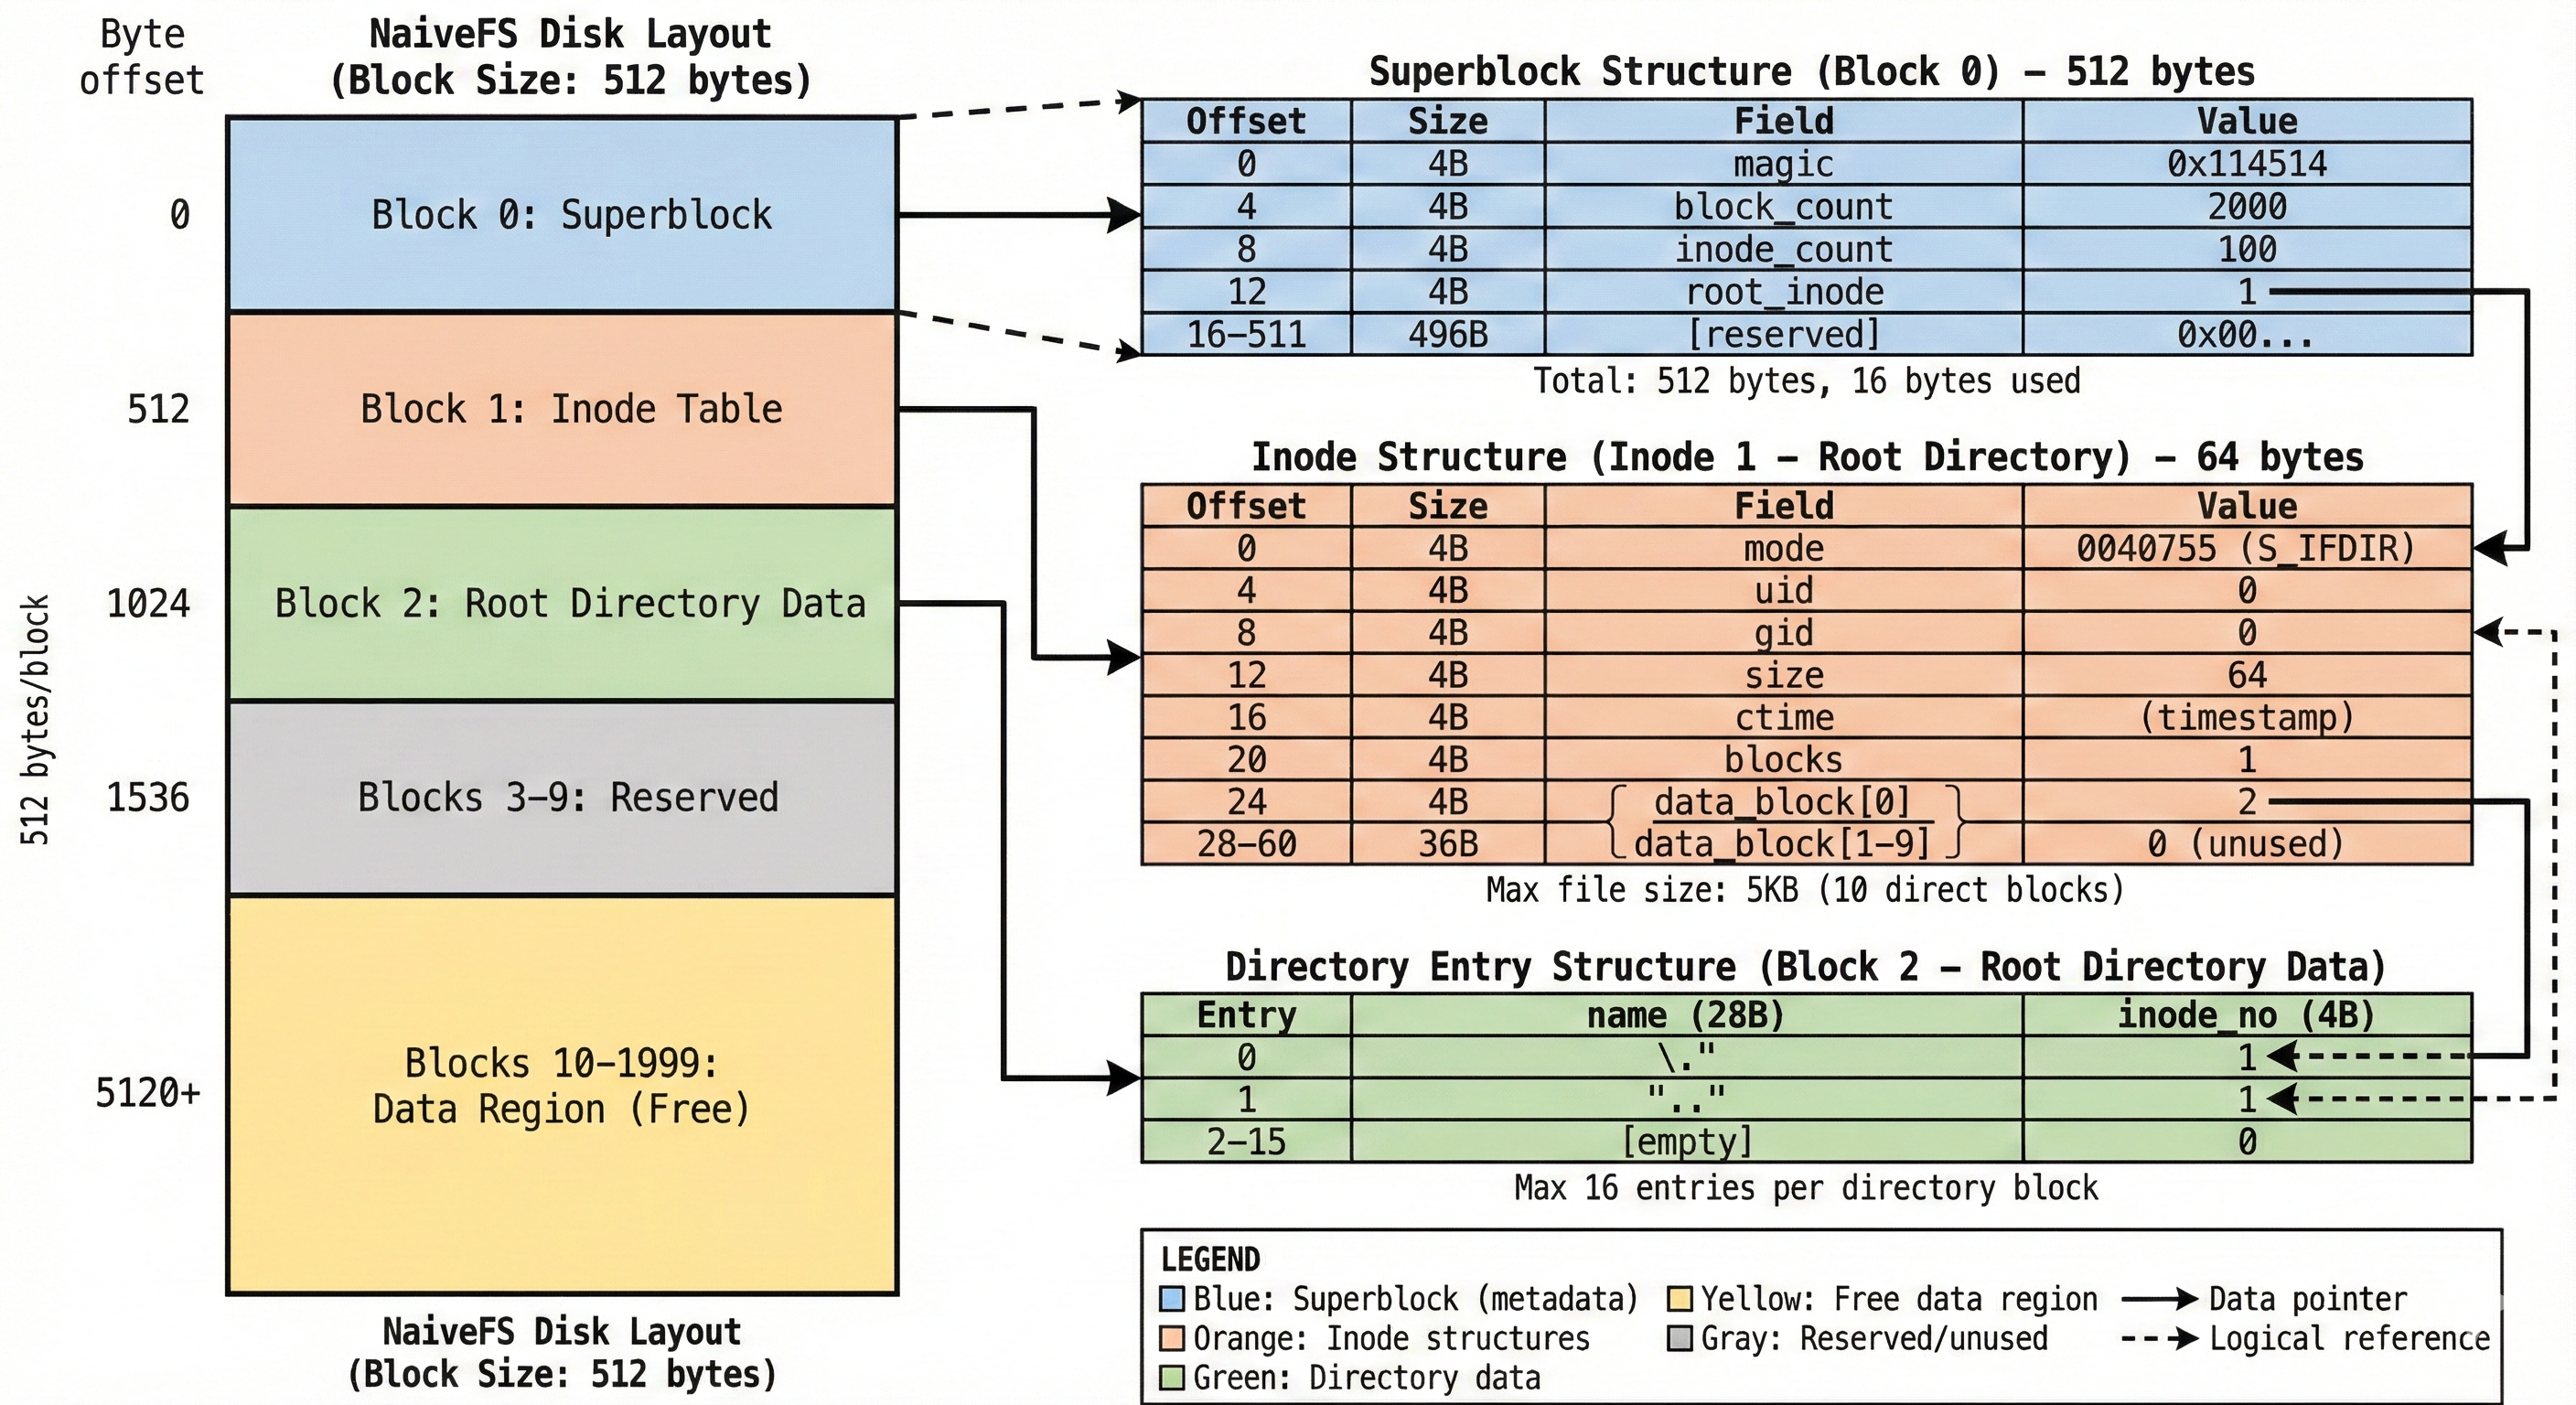
\includegraphics[width=0.95\textwidth]{img/fs.png}
  \end{center}
  \caption{格式化后的磁盘布局(图片由 Nano Banana Pro 生成,可能存在错误)}
\end{figure}


\subsubsection{内核模块实现}

\par 内核模块是文件系统的核心,它向 Linux VFS(虚拟文件系统)层注册我们的文件系统类型,并实现各种文件操作的回调函数。

\paragraph{适配 Linux 6.18 内核的新挂载 API}

\par Linux 内核在持续演进过程中,对文件系统挂载机制进行了重构。传统的挂载 API 使用 \texttt{.mount} 回调函数,而新版内核(6.x 系列)引入了基于 \texttt{fs\_context} 的新挂载 API,提供了更灵活的挂载参数解析和错误处理机制。

\begin{lstlisting}[language=C]
#include <linux/fs_context.h>

static const struct fs_context_operations naive_context_ops = {
    .get_tree = naive_get_tree,
};

static int naive_init_fs_context(struct fs_context *fc) {
    fc->ops = &naive_context_ops;
    return 0;
}

static int naive_get_tree(struct fs_context *fc) {
    return get_tree_bdev(fc, naive_fill_super);
}

static struct file_system_type naive_fs_type = {
    .owner = THIS_MODULE,
    .name = "naive",
    .init_fs_context = naive_init_fs_context,  // 替代旧版的 .mount
    .kill_sb = kill_block_super,
    .fs_flags = FS_REQUIRES_DEV,
};
\end{lstlisting}

\par 挂载流程的调用链如下:当用户执行 \texttt{mount} 命令时,内核首先调用 \texttt{init\_fs\_context} 初始化上下文并设置操作表,随后调用 \texttt{get\_tree} 执行实际的挂载操作。\texttt{get\_tree\_bdev} 是内核提供的辅助函数,专门用于块设备文件系统的挂载,它会打开块设备并调用我们提供的 \texttt{naive\_fill\_super} 函数填充超级块。
\paragraph{超级块填充函数}

\par \texttt{naive\_fill\_super} 函数在挂载时被调用,负责读取磁盘上的超级块、验证魔数、创建根 inode:

\begin{lstlisting}[language=C]
static int naive_fill_super(struct super_block *sb, struct fs_context *fc) {
    struct buffer_head *bh;
    struct naive_super_block *nsb;
    struct naive_inode root_ni;
    struct inode *root;

    if (!sb_set_blocksize(sb, NAIVE_BLOCK_SIZE)) return -EINVAL;
    
    // 必须在 new_inode() 之前设置 s_op
    sb->s_magic = NAIVE_MAGIC;
    sb->s_op = &naive_sb_ops;
    
    // 读取并验证超级块
    bh = sb_bread(sb, 0);
    if (!bh) return -EIO;
    nsb = (struct naive_super_block *)bh->b_data;
    
    if (nsb->magic != NAIVE_MAGIC) {
        printk(KERN_ERR "NaiveFS: Magic mismatch.\n");
        brelse(bh);
        return -EINVAL;
    }
    brelse(bh);

    // 读取根目录 inode 并创建 VFS inode
    naive_read_inode_from_disk(sb, 1, &root_ni);
    root = new_inode(sb);
    if (!root) return -ENOMEM;
    
    root->i_ino = 1;
    root->i_sb = sb;
    naive_fill_inode(root, &root_ni);
    
    sb->s_root = d_make_root(root);
    return sb->s_root ? 0 : -ENOMEM;
}
\end{lstlisting}

\par 需要特别注意的是, \texttt{sb->s\_op} 必须在调用 \texttt{new\_inode()} 之前设置。 这是因为 \texttt{new\_inode()} 内部会通过 \texttt{sb->s\_op->alloc\_inode} 分配 inode 结构体,若 \texttt{s\_op} 为 NULL 将导致内核空指针解引用崩溃。

\paragraph{Linux 6.18 的 API 变化}

\par Linux 6.18 内核对文件系统相关的多个回调函数签名进行了修改,主要变化包括:

\par \textbf{1. 写入操作回调函数}:\texttt{address\_space\_operations} 中的 \texttt{write\_begin} 和 \texttt{write\_end} 的第一个参数从 \texttt{struct file *} 改为 \texttt{const struct kiocb *}:

\begin{lstlisting}[language=C]
// Linux 6.18+ 新签名
static int naive_write_begin(const struct kiocb *iocb, 
                             struct address_space *mapping,
                             loff_t pos, unsigned len,
                             struct folio **foliop, void **fsdata) {
    return block_write_begin(mapping, pos, len, foliop, naive_get_block);
}

static int naive_write_end(const struct kiocb *iocb,
                           struct address_space *mapping,
                           loff_t pos, unsigned len, unsigned copied,
                           struct folio *folio, void *fsdata) {
    struct inode *inode = mapping->host;
    int ret 
    = generic_write_end(iocb, mapping, pos, len, copied, folio, fsdata);
    // 更新磁盘上的文件大小
    if (ret > 0) {
        struct naive_inode ni;
        naive_read_inode_from_disk(inode->i_sb, inode->i_ino, &ni);
        ni.size = i_size_read(inode);
        naive_write_inode_to_disk(inode->i_sb, inode->i_ino, &ni);
    }
    return ret;
}
\end{lstlisting}

\par \textbf{2. 目录创建回调函数}:\texttt{inode\_operations} 中的 \texttt{mkdir} 返回值从 \texttt{int} 改为 \texttt{struct dentry *},成功时返回 \texttt{NULL},失败时返回 \texttt{ERR\_PTR(err)}:

\begin{lstlisting}[language=C]
// Linux 6.18+ 新签名
static struct dentry *naive_mkdir(struct mnt_idmap *idmap, struct inode *dir,
                                  struct dentry *dentry, umode_t mode) {
    // ... 创建目录的逻辑 ...
    
    if (err) return ERR_PTR(err);
    
    d_instantiate(dentry, inode);
    return NULL;  // 成功返回 NULL
}
\end{lstlisting}

\par \textbf{3. 已移除的函数}:\texttt{generic\_drop\_inode} 在 6.18 内核中已不存在,\texttt{super\_operations} 中的 \texttt{drop\_inode} 字段可以省略或使用其他替代方案。

\paragraph{目录操作实现}

\par 目录遍历通过 \texttt{iterate\_shared} 回调实现,用于支持 \texttt{ls} 命令:

\begin{lstlisting}[language=C]
static int naive_iterate(struct file *filp, struct dir_context *ctx) {
    struct inode *inode = file_inode(filp);
    struct naive_inode ni;
    struct buffer_head *bh;
    struct naive_dir_entry *de;
    
    naive_read_inode_from_disk(inode->i_sb, inode->i_ino, &ni);
    bh = sb_bread(inode->i_sb, ni.data_block[0]);
    de = (struct naive_dir_entry *)bh->b_data;
    
    for (int i = 0; i < NAIVE_BLOCK_SIZE / sizeof(struct naive_dir_entry); i++) {
        if (de[i].inode_no != 0) {
            dir_emit(ctx, de[i].name, strlen(de[i].name), 
                     de[i].inode_no, DT_UNKNOWN);
        }
        ctx->pos += sizeof(struct naive_dir_entry);
    }
    brelse(bh);
    return 0;
}
\end{lstlisting}

\par 文件查找通过 \texttt{lookup} 回调实现,当访问目录中的某个文件时被调用:

\begin{lstlisting}[language=C]
static struct dentry *naive_lookup(struct inode *dir, struct dentry *dentry, 
                                   unsigned int flags) {
    // 读取目录数据块,遍历查找匹配的文件名
    // 找到后通过 iget_locked 获取或创建 VFS inode
    // 调用 d_splice_alias 将 dentry 与 inode 关联
}
\end{lstlisting}

\subsubsection{编译与测试}

\par 内核模块的编译需要通过 Makefile 调用内核构建系统:

\begin{lstlisting}[language=make]
obj-m := naive_fs.o
KDIR := /lib/modules/$(shell uname -r)/build

all:
	make -C $(KDIR) M=$(PWD) modules

clean:
	make -C $(KDIR) M=$(PWD) clean
\end{lstlisting}

\par 完整的编译和测试流程如下:

\begin{lstlisting}[language=bash]
# 编译格式化工具和内核模块
gcc mkfs.naive.c -o mkfs.naive
make

# 格式化虚拟块设备
sudo ./mkfs.naive /dev/loop0

# 加载内核模块并挂载
sudo insmod naive_fs.ko
mkdir -p mnt
sudo mount -t naive /dev/loop0 mnt

# 验证挂载结果
ls -la mnt/
mount | grep naive
df -T mnt/
\end{lstlisting}

\par 执行 \texttt{ls -la mnt/} 列出挂载点目录的内容,结果如下:

\begin{lstlisting}
total 0
drwxr-xr-x 1 root root  64 Jan  6 20:45 .
drwxr-xr-x 1 huhu huhu 574 Jan  6 20:45 ..
\end{lstlisting}

\par 输出显示了两个条目:\texttt{.} 代表当前目录,\texttt{..} 代表父目录。这两个特殊目录项是我们在格式化工具中预先写入的,它们的存在证明格式化程序正确地初始化了根目录的数据块,内核模块也成功地解析并展示了这些目录项。

\par 执行 \texttt{mount | grep naive} 查询系统挂载表:

\begin{lstlisting}
/dev/loop0 on /home/huhu/fs/mnt type naive (rw,relatime)
\end{lstlisting}

\par 输出表明 loop0 设备已成功以 naive 文件系统类型挂载到指定目录,且挂载选项包含 \texttt{rw}(读写模式)和 \texttt{relatime}(访问时间优化),说明内核正确识别了我们注册的文件系统类型。

\par 执行 \texttt{df -T mnt/} 查看文件系统类型和磁盘空间:

\begin{lstlisting}
Filesystem     Type  1K-blocks  Used Available Use% Mounted on
/dev/loop0     naive         0     0         0    - /home/huhu/fs/mnt
\end{lstlisting}

\par Type 列显示 \texttt{naive},确认了文件系统类型。容量显示为 0 是因为我们使用了简化的 \texttt{simple\_statfs} 函数,若需显示正确的磁盘容量,需要实现自定义的 statfs 回调。

\par 测试文件系统的完整功能:

\begin{lstlisting}[language=bash]
# 测试文件创建
sudo touch mnt/hello.txt
ls -la mnt/

# 测试目录创建
sudo mkdir mnt/subdir
ls -la mnt/

# 测试文件写入和读取
sudo sh -c 'echo "Hello NaiveFS" > mnt/hello.txt'
cat mnt/hello.txt

# 测试文件和目录删除
sudo rm mnt/hello.txt
sudo rmdir mnt/subdir
ls -la mnt/
\end{lstlisting}

\par 创建文件后执行 \texttt{ls -la mnt/}:

\begin{lstlisting}
total 0
drwxr-xr-x 1 root root  96 Jan  6 20:45 .
drwxr-xr-x 1 huhu huhu 574 Jan  6 20:45 ..
-rw-r--r-- 1 root root   0 Jan  6 20:48 hello.txt
\end{lstlisting}

\par 创建目录后执行 \texttt{ls -la mnt/}:

\begin{lstlisting}
total 0
drwxr-xr-x 1 root root 128 Jan  6 20:45 .
drwxr-xr-x 1 huhu huhu 574 Jan  6 20:45 ..
-rw-r--r-- 1 root root   0 Jan  6 20:48 hello.txt
drwxr-xr-x 1 root root  64 Jan  6 20:48 subdir
\end{lstlisting}

\par 文件写入和读取测试:

\begin{lstlisting}
$ cat mnt/hello.txt
Hello NaiveFS
\end{lstlisting}

\par 删除文件和目录后执行 \texttt{ls -la mnt/}:

\begin{lstlisting}
total 0
drwxr-xr-x 0 root root 128 Jan  6 20:45 .
drwxr-xr-x 1 huhu huhu 574 Jan  6 20:45 ..
\end{lstlisting}

\par 查看内核日志 \texttt{dmesg | tail -20}(相关部分):

\begin{lstlisting}
NaiveFS: Module loaded
NaiveFS: Mounted successfully. Magic matches.
NaiveFS: Created file 'hello.txt' (inode 2)
NaiveFS: Created directory 'subdir' (inode 3, data block 10)
NaiveFS: Removed file 'hello.txt'
NaiveFS: Removed directory 'subdir'
\end{lstlisting}

\par 内核日志清晰地记录了文件系统的各项操作:模块加载、挂载成功(魔数校验通过)、创建文件(分配 inode 2)、创建目录(分配 inode 3,数据块位于 Block 10)、删除文件和删除目录。这些日志信息是我们在内核模块中通过 \texttt{printk} 输出的,便于调试和验证。

\par 清理环境:

\begin{lstlisting}[language=bash]
sudo umount mnt
sudo rmmod naive_fs
sudo losetup -d /dev/loop0
\end{lstlisting}

\subsection{实验总结}

\par 本实验成功实现了一个具备完整功能的简易文件系统 NaiveFS,包括设备创建、分区格式化、文件系统注册、目录操作(创建、删除、遍历)和文件操作(创建、读写、删除)。实验过程中,我们深入理解了 Linux VFS 层的抽象机制,掌握了内核模块开发的基本方法,并针对 Linux 6.18 内核的 API 变化进行了适配。

\par 通过这个实验,我们认识到文件系统的核心是数据结构的设计与管理:超级块提供全局元信息,inode 描述文件属性,目录项建立名称到 inode 的映射,数据块存储实际内容。VFS 层通过一组标准化的操作表(\texttt{super\_operations}、\texttt{inode\_operations}、\texttt{file\_operations}、\texttt{address\_space\_operations})将具体文件系统的实现与上层系统调用解耦,这种设计使得 Linux 能够支持数十种不同的文件系统。
